\documentclass[]{article}
\usepackage[margin=1in]{geometry}
\usepackage{dcolumn}
\usepackage{graphicx}
\usepackage{hyperref}
\hypersetup{
	colorlinks = true,
	urlcolor = black
}

\title{\LaTeX~Tables for Bitcoin Mining Stock Analysis}
\author{Tim Dombrowski}
\date{\today}

\begin{document}

\maketitle

\large

\section{Data Work and Project Background}

See the \href{https://github.com/tim-dombrowski/bitcoin-miningstocks-project/blob/main/R\%20Notebook/miningstocks.Rmd}{miningstocks.Rmd} R Notebook for a detailed write-up of the data work to generate these tables. More broadly, see \href{https://github.com/tim-dombrowski/bitcoin-miningstocks-project}{this project's GitHub repository} for more details on the project background and how to replicate the analysis.

\section{Summary Statistics}

\subsection{Nominal Returns}


% Table created by stargazer v.5.2.3 by Marek Hlavac, Social Policy Institute. E-mail: marek.hlavac at gmail.com
% Date and time: Tue, Apr 23, 2024 - 18:53:04
\begin{table}[!htbp] \centering 
  \caption{Summary Statistics for the Final Monthly Dataset. Asset nominal returns and growth rates are all annualized and measured in percentage units. Table generated with the stargazer R package (Hlavac, 2022).} 
  \label{SummaryStats_nominal} 
\large 
\begin{tabular}{@{\extracolsep{5pt}}lrrrrr} 
\\[-1.8ex]\hline 
\hline \\[-1.8ex] 
Statistic & \multicolumn{1}{c}{N} & \multicolumn{1}{c}{Mean} & \multicolumn{1}{c}{St. Dev.} & \multicolumn{1}{c}{Min} & \multicolumn{1}{c}{Max} \\ 
\hline \\[-1.8ex] 
INF & 32 & 5.174 & 3.736 & $-$0.077 & 14.887 \\ 
RF & 32 & 3.208 & 1.041 & 1.283 & 4.798 \\ 
BTC & 32 & 20.199 & 218.832 & $-$569.177 & 435.210 \\ 
MARA & 32 & $-$7.569 & 497.362 & $-$875.587 & 1,066.745 \\ 
CLSK & 32 & 16.942 & 416.996 & $-$774.014 & 877.120 \\ 
RIOT & 32 & $-$37.136 & 409.067 & $-$883.316 & 737.936 \\ 
CIFR & 32 & $-$24.583 & 389.626 & $-$687.697 & 914.568 \\ 
HUT & 32 & $-$28.569 & 429.338 & $-$781.097 & 984.047 \\ 
BTDR & 32 & $-$12.165 & 361.266 & $-$1,136.203 & 987.126 \\ 
SPY & 32 & 8.149 & 64.095 & $-$116.402 & 105.709 \\ 
Hashrate & 32 & 67.230 & 60.657 & $-$64.583 & 227.352 \\ 
Difficulty & 32 & 65.153 & 55.612 & $-$56.532 & 198.738 \\ 
\hline \\[-1.8ex] 
\end{tabular} 
\end{table} 


\pagebreak

\subsection{Real Returns}


% Table created by stargazer v.5.2.3 by Marek Hlavac, Social Policy Institute. E-mail: marek.hlavac at gmail.com
% Date and time: Thu, Apr 03, 2025 - 19:02:50
% Requires LaTeX packages: dcolumn 
\begin{table}[!htbp] \centering 
  \caption{Summary Statistics for the Final Monthly Dataset. Asset real returns and growth rates are all annualized and measured in percentage units. Table generated with the stargazer R package (Hlavac, 2022).} 
  \label{SummaryStats_real} 
\large 
\begin{tabular}{@{\extracolsep{5pt}}lD{.}{.}{-2} D{.}{.}{-2} D{.}{.}{-2} D{.}{.}{-2} D{.}{.}{-2} } 
\\[-1.8ex]\hline 
\hline \\[-1.8ex] 
Statistic & \multicolumn{1}{c}{N} & \multicolumn{1}{c}{Mean} & \multicolumn{1}{c}{St. Dev.} & \multicolumn{1}{c}{Min} & \multicolumn{1}{c}{Max} \\ 
\hline \\[-1.8ex] 
RF & 43 & -0.87 & 3.84 & -10.65 & 4.34 \\ 
BTC & 43 & 16.18 & 194.39 & -506.41 & 410.95 \\ 
MARA & 43 & -19.57 & 437.31 & -853.49 & 1,073.04 \\ 
CLSK & 43 & -17.48 & 367.56 & -744.09 & 832.84 \\ 
RIOT & 43 & -35.34 & 354.29 & -848.54 & 686.06 \\ 
CIFR & 43 & -24.17 & 355.38 & -609.08 & 851.75 \\ 
HUT & 43 & -13.57 & 403.91 & -740.25 & 916.93 \\ 
BTDR & 43 & 2.22 & 363.06 & -1,125.04 & 954.50 \\ 
SPY & 43 & 5.59 & 56.08 & -115.61 & 106.82 \\ 
Hashrate & 43 & 58.31 & 58.59 & -64.58 & 227.35 \\ 
Difficulty & 43 & 57.13 & 54.70 & -56.53 & 198.74 \\ 
\hline \\[-1.8ex] 
\end{tabular} 
\end{table} 


%\pagebreak

\subsection{Excess Returns}


% Table created by stargazer v.5.2.3 by Marek Hlavac, Social Policy Institute. E-mail: marek.hlavac at gmail.com
% Date and time: Tue, Apr 23, 2024 - 18:53:10
\begin{table}[!htbp] \centering 
  \caption{Summary Statistics for the Final Monthly Dataset. Asset excess returns and growth rates are all annualized and measured in percentage units. Table generated with the stargazer R package (Hlavac, 2022).} 
  \label{SummaryStats_excess} 
\large 
\begin{tabular}{@{\extracolsep{5pt}}lrrrrr} 
\\[-1.8ex]\hline 
\hline \\[-1.8ex] 
Statistic & \multicolumn{1}{c}{N} & \multicolumn{1}{c}{Mean} & \multicolumn{1}{c}{St. Dev.} & \multicolumn{1}{c}{Min} & \multicolumn{1}{c}{Max} \\ 
\hline \\[-1.8ex] 
BTC & 32 & 18.141 & 203.464 & $-$498.161 & 409.336 \\ 
MARA & 32 & $-$6.704 & 475.113 & $-$852.552 & 1,064.672 \\ 
CLSK & 32 & 14.270 & 392.870 & $-$739.470 & 829.032 \\ 
RIOT & 32 & $-$35.049 & 388.384 & $-$843.524 & 691.630 \\ 
CIFR & 32 & $-$21.932 & 368.702 & $-$601.323 & 857.974 \\ 
HUT & 32 & $-$26.870 & 406.255 & $-$739.560 & 923.406 \\ 
BTDR & 32 & $-$15.319 & 353.164 & $-$1,130.279 & 959.196 \\ 
SPY & 32 & 4.985 & 60.870 & $-$114.656 & 102.893 \\ 
Hashrate & 32 & 67.230 & 60.657 & $-$64.583 & 227.352 \\ 
Difficulty & 32 & 65.153 & 55.612 & $-$56.532 & 198.738 \\ 
\hline \\[-1.8ex] 
\end{tabular} 
\end{table} 


\pagebreak

\subsection{Nominal Return Correlations}

\begin{figure}[htbp]
	\label{finalcorplot}
	\caption{Correlation Matrix Heatmap for Nominal Monthly Returns}
	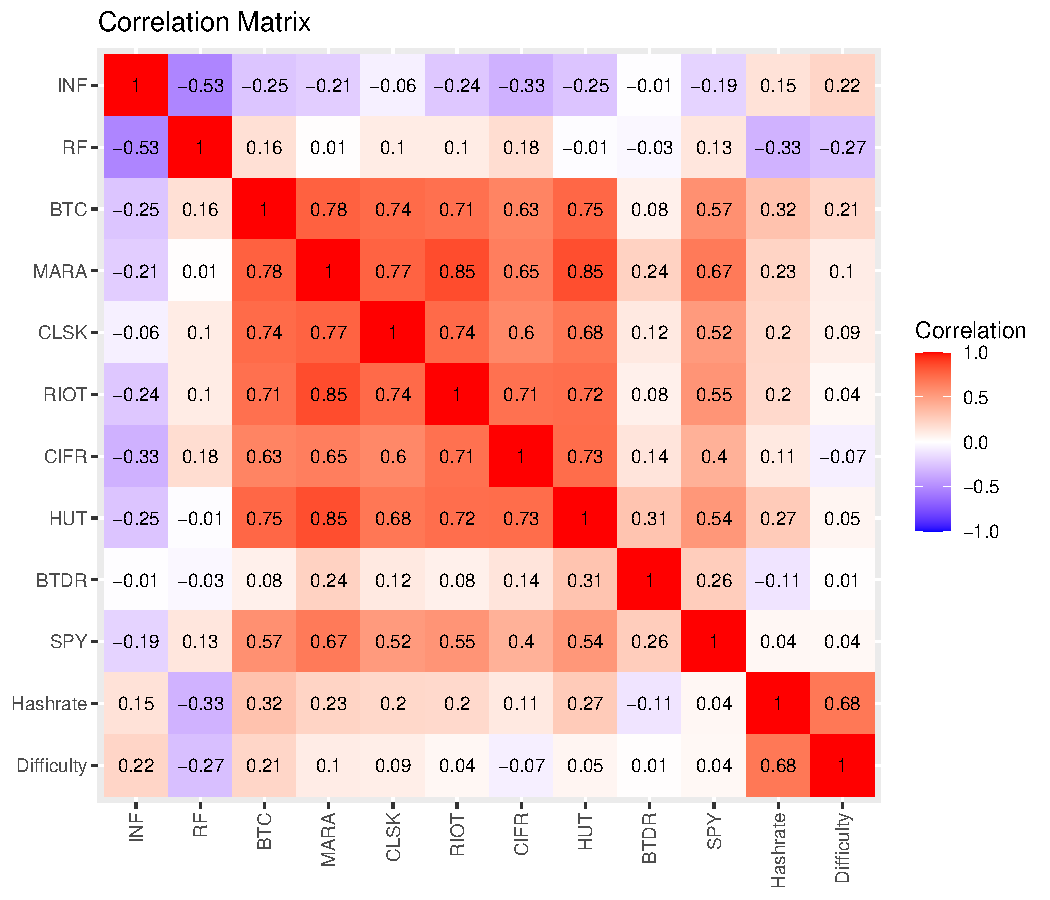
\includegraphics[width=\linewidth]{finalcorplot.pdf}
\end{figure}

%%%%%%%%%%%%%%%%%%%%%%%%%%%%%%%%%%%
\pagebreak
%%%%%%%%%%%%%%%%%%%%%%%%%%%%%%%%%%%

\section{Model Results}

\subsection{Marathon Digital Holdings (MARA)}


% Table created by stargazer v.5.2.3 by Marek Hlavac, Social Policy Institute. E-mail: marek.hlavac at gmail.com
% Date and time: Thu, Apr 03, 2025 - 19:10:11
% Requires LaTeX packages: dcolumn 
\begin{table}[!htbp] \centering 
  \caption{Factor Model Results for Marathon Digital Holdings (MARA). Table generated with the stargazer R package (Hlavac, 2022).} 
  \label{ModelResults_MARA} 
\large 
\begin{tabular}{@{\extracolsep{5pt}}lD{.}{.}{-2} D{.}{.}{-2} D{.}{.}{-2} D{.}{.}{-2} D{.}{.}{-2} } 
\\[-1.8ex]\hline 
\hline \\[-1.8ex] 
 & \multicolumn{5}{c}{\textit{Dependent variable:}} \\ 
\cline{2-6} 
\\[-1.8ex] & \multicolumn{5}{c}{MARA} \\ 
\\[-1.8ex] & \multicolumn{1}{c}{(1)} & \multicolumn{1}{c}{(2)} & \multicolumn{1}{c}{(3)} & \multicolumn{1}{c}{(4)} & \multicolumn{1}{c}{(5)}\\ 
\hline \\[-1.8ex] 
 SPY & 5.26^{***} & 2.64^{***} & 2.69^{***} & 2.60^{***} & 2.70^{***} \\ 
  & (0.91) & (0.85) & (0.88) & (0.87) & (0.88) \\ 
  & & & & & \\ 
 BTC &  & 1.29^{***} & 1.26^{***} & 1.32^{***} & 1.26^{***} \\ 
  &  & (0.24) & (0.26) & (0.25) & (0.26) \\ 
  & & & & & \\ 
 Hashrate &  &  & 0.23 &  & 0.80 \\ 
  &  &  & (0.75) &  & (1.00) \\ 
  & & & & & \\ 
 Difficulty &  &  &  & -0.35 & -0.89 \\ 
  &  &  &  & (0.77) & (1.03) \\ 
  & & & & & \\ 
 Constant & -71.16 & -70.78^{*} & -84.14 & -51.05 & -66.59 \\ 
  & (53.04) & (40.87) & (60.12) & (60.33) & (63.69) \\ 
  & & & & & \\ 
\hline \\[-1.8ex] 
Observations & \multicolumn{1}{c}{43} & \multicolumn{1}{c}{43} & \multicolumn{1}{c}{43} & \multicolumn{1}{c}{43} & \multicolumn{1}{c}{43} \\ 
R$^{2}$ & \multicolumn{1}{c}{0.45} & \multicolumn{1}{c}{0.68} & \multicolumn{1}{c}{0.68} & \multicolumn{1}{c}{0.68} & \multicolumn{1}{c}{0.69} \\ 
Adjusted R$^{2}$ & \multicolumn{1}{c}{0.44} & \multicolumn{1}{c}{0.66} & \multicolumn{1}{c}{0.66} & \multicolumn{1}{c}{0.66} & \multicolumn{1}{c}{0.65} \\ 
\hline 
\hline \\[-1.8ex] 
\textit{Note:}  & \multicolumn{5}{r}{$^{*}$p$<$0.1; $^{**}$p$<$0.05; $^{***}$p$<$0.01} \\ 
\end{tabular} 
\end{table} 


\pagebreak

\subsection{Cleanspark (CLSK)}


% Table created by stargazer v.5.2.3 by Marek Hlavac, Social Policy Institute. E-mail: marek.hlavac at gmail.com
% Date and time: Tue, Apr 23, 2024 - 18:51:19
\begin{table}[!htbp] \centering 
  \caption{Factor Model Results for Cleanspark (CLSK). Table generated with the stargazer R package (Hlavac, 2022).} 
  \label{ModelResults_CLSK} 
\large 
\begin{tabular}{@{\extracolsep{5pt}}lccccc} 
\\[-1.8ex]\hline 
\hline \\[-1.8ex] 
 & \multicolumn{5}{c}{\textit{Dependent variable:}} \\ 
\cline{2-6} 
\\[-1.8ex] & \multicolumn{5}{c}{CLSK} \\ 
\\[-1.8ex] & (1) & (2) & (3) & (4) & (5)\\ 
\hline \\[-1.8ex] 
 SPY & 3.413$^{***}$ & 1.062 & 1.028 & 1.018 & 1.016 \\ 
  & (1.011) & (0.964) & (0.982) & (0.980) & (0.999) \\ 
  & & & & & \\ 
 BTC &  & 1.231$^{***}$ & 1.278$^{***}$ & 1.269$^{***}$ & 1.273$^{***}$ \\ 
  &  & (0.282) & (0.309) & (0.294) & (0.314) \\ 
  & & & & & \\ 
 Hashrate &  &  & $-$0.384 &  & $-$0.065 \\ 
  &  &  & (0.935) &  & (1.329) \\ 
  & & & & & \\ 
 Difficulty &  &  &  & $-$0.517 & $-$0.470 \\ 
  &  &  &  & (0.962) & (1.371) \\ 
  & & & & & \\ 
 Constant & $-$10.871 & $-$16.583 & 8.558 & 16.713 & 17.947 \\ 
  & (64.326) & (50.873) & (80.061) & (80.558) & (85.836) \\ 
  & & & & & \\ 
\hline \\[-1.8ex] 
Observations & 32 & 32 & 32 & 32 & 32 \\ 
R$^{2}$ & 0.275 & 0.562 & 0.565 & 0.567 & 0.567 \\ 
Adjusted R$^{2}$ & 0.251 & 0.532 & 0.518 & 0.520 & 0.502 \\ 
\hline 
\hline \\[-1.8ex] 
\textit{Note:}  & \multicolumn{5}{r}{$^{*}$p$<$0.1; $^{**}$p$<$0.05; $^{***}$p$<$0.01} \\ 
\end{tabular} 
\end{table} 


\pagebreak

\subsection{Riot Blockchain (RIOT)}


% Table created by stargazer v.5.2.3 by Marek Hlavac, Social Policy Institute. E-mail: marek.hlavac at gmail.com
% Date and time: Thu, Apr 03, 2025 - 19:02:53
% Requires LaTeX packages: dcolumn 
\begin{table}[!htbp] \centering 
  \caption{Factor Model Results for Riot Blockchain (RIOT). Table generated with the stargazer R package (Hlavac, 2022).} 
  \label{ModelResults_RIOT} 
\large 
\begin{tabular}{@{\extracolsep{5pt}}lD{.}{.}{-2} D{.}{.}{-2} D{.}{.}{-2} D{.}{.}{-2} D{.}{.}{-2} } 
\\[-1.8ex]\hline 
\hline \\[-1.8ex] 
 & \multicolumn{5}{c}{\textit{Dependent variable:}} \\ 
\cline{2-6} 
\\[-1.8ex] & \multicolumn{5}{c}{RIOT} \\ 
\\[-1.8ex] & \multicolumn{1}{c}{(1)} & \multicolumn{1}{c}{(2)} & \multicolumn{1}{c}{(3)} & \multicolumn{1}{c}{(4)} & \multicolumn{1}{c}{(5)}\\ 
\hline \\[-1.8ex] 
 SPY & 3.49^{***} & 1.32 & 1.32 & 1.25 & 1.34 \\ 
  & (0.84) & (0.83) & (0.86) & (0.84) & (0.86) \\ 
  & & & & & \\ 
 BTC &  & 1.07^{***} & 1.07^{***} & 1.12^{***} & 1.07^{***} \\ 
  &  & (0.23) & (0.25) & (0.24) & (0.25) \\ 
  & & & & & \\ 
 Hashrate &  &  & -0.01 &  & 0.72 \\ 
  &  &  & (0.74) &  & (0.98) \\ 
  & & & & & \\ 
 Difficulty &  &  &  & -0.66 & -1.15 \\ 
  &  &  &  & (0.75) & (1.00) \\ 
  & & & & & \\ 
 Constant & -69.90 & -69.58^{*} & -68.86 & -32.16 & -46.18 \\ 
  & (48.69) & (39.96) & (58.86) & (58.57) & (61.91) \\ 
  & & & & & \\ 
\hline \\[-1.8ex] 
Observations & \multicolumn{1}{c}{43} & \multicolumn{1}{c}{43} & \multicolumn{1}{c}{43} & \multicolumn{1}{c}{43} & \multicolumn{1}{c}{43} \\ 
R$^{2}$ & \multicolumn{1}{c}{0.30} & \multicolumn{1}{c}{0.54} & \multicolumn{1}{c}{0.54} & \multicolumn{1}{c}{0.55} & \multicolumn{1}{c}{0.55} \\ 
Adjusted R$^{2}$ & \multicolumn{1}{c}{0.28} & \multicolumn{1}{c}{0.52} & \multicolumn{1}{c}{0.50} & \multicolumn{1}{c}{0.51} & \multicolumn{1}{c}{0.51} \\ 
\hline 
\hline \\[-1.8ex] 
\textit{Note:}  & \multicolumn{5}{r}{$^{*}$p$<$0.1; $^{**}$p$<$0.05; $^{***}$p$<$0.01} \\ 
\end{tabular} 
\end{table} 


\pagebreak

\subsection{Cipher Mining (CIFR)}


% Table created by stargazer v.5.2.3 by Marek Hlavac, Social Policy Institute. E-mail: marek.hlavac at gmail.com
% Date and time: Tue, Jul 09, 2024 - 16:40:32
% Requires LaTeX packages: dcolumn 
\begin{table}[!htbp] \centering 
  \caption{Factor Model Results for Cipher Mining (CIFR). Table generated with the stargazer R package (Hlavac, 2022).} 
  \label{ModelResults_CIFR} 
\large 
\begin{tabular}{@{\extracolsep{5pt}}lD{.}{.}{-2} D{.}{.}{-2} D{.}{.}{-2} D{.}{.}{-2} D{.}{.}{-2} } 
\\[-1.8ex]\hline 
\hline \\[-1.8ex] 
 & \multicolumn{5}{c}{\textit{Dependent variable:}} \\ 
\cline{2-6} 
\\[-1.8ex] & \multicolumn{5}{c}{CIFR} \\ 
\\[-1.8ex] & \multicolumn{1}{c}{(1)} & \multicolumn{1}{c}{(2)} & \multicolumn{1}{c}{(3)} & \multicolumn{1}{c}{(4)} & \multicolumn{1}{c}{(5)}\\ 
\hline \\[-1.8ex] 
 SPY & 2.38^{**} & 0.43 & 0.39 & 0.33 & 0.36 \\ 
  & (0.98) & (1.05) & (1.08) & (1.06) & (1.08) \\ 
  & & & & & \\ 
 BTC &  & 0.99^{***} & 1.03^{***} & 1.06^{***} & 1.01^{***} \\ 
  &  & (0.31) & (0.33) & (0.32) & (0.34) \\ 
  & & & & & \\ 
 Hashrate &  &  & -0.28 &  & 0.72 \\ 
  &  &  & (0.96) &  & (1.39) \\ 
  & & & & & \\ 
 Difficulty &  &  &  & -0.93 & -1.49 \\ 
  &  &  &  & (1.01) & (1.49) \\ 
  & & & & & \\ 
 Constant & -53.67 & -55.13 & -37.51 & 2.50 & -7.80 \\ 
  & (61.74) & (54.32) & (81.38) & (83.32) & (86.64) \\ 
  & & & & & \\ 
\hline \\[-1.8ex] 
Observations & \multicolumn{1}{c}{34} & \multicolumn{1}{c}{34} & \multicolumn{1}{c}{34} & \multicolumn{1}{c}{34} & \multicolumn{1}{c}{34} \\ 
R$^{2}$ & \multicolumn{1}{c}{0.16} & \multicolumn{1}{c}{0.37} & \multicolumn{1}{c}{0.37} & \multicolumn{1}{c}{0.38} & \multicolumn{1}{c}{0.39} \\ 
Adjusted R$^{2}$ & \multicolumn{1}{c}{0.13} & \multicolumn{1}{c}{0.33} & \multicolumn{1}{c}{0.31} & \multicolumn{1}{c}{0.32} & \multicolumn{1}{c}{0.31} \\ 
\hline 
\hline \\[-1.8ex] 
\textit{Note:}  & \multicolumn{5}{r}{$^{*}$p$<$0.1; $^{**}$p$<$0.05; $^{***}$p$<$0.01} \\ 
\end{tabular} 
\end{table} 


\pagebreak

\subsection{Hut 8 Mining (HUT)}


% Table created by stargazer v.5.2.3 by Marek Hlavac, Social Policy Institute. E-mail: marek.hlavac at gmail.com
% Date and time: Tue, Apr 23, 2024 - 18:51:22
\begin{table}[!htbp] \centering 
  \caption{Factor Model Results for Hut 8 Mining (HUT). Table generated with the stargazer R package (Hlavac, 2022).} 
  \label{ModelResults_HUT} 
\large 
\begin{tabular}{@{\extracolsep{5pt}}lccccc} 
\\[-1.8ex]\hline 
\hline \\[-1.8ex] 
 & \multicolumn{5}{c}{\textit{Dependent variable:}} \\ 
\cline{2-6} 
\\[-1.8ex] & \multicolumn{5}{c}{HUT} \\ 
\\[-1.8ex] & (1) & (2) & (3) & (4) & (5)\\ 
\hline \\[-1.8ex] 
 SPY & 3.471$^{***}$ & 0.873 & 0.984 & 0.845 & 0.926 \\ 
  & (1.046) & (0.950) & (0.939) & (0.968) & (0.897) \\ 
  & & & & & \\ 
 BTC &  & 1.361$^{***}$ & 1.210$^{***}$ & 1.384$^{***}$ & 1.183$^{***}$ \\ 
  &  & (0.278) & (0.295) & (0.291) & (0.282) \\ 
  & & & & & \\ 
 Hashrate &  &  & 1.230 &  & 2.836$^{**}$ \\ 
  &  &  & (0.894) &  & (1.195) \\ 
  & & & & & \\ 
 Difficulty &  &  &  & $-$0.321 & $-$2.368$^{*}$ \\ 
  &  &  &  & (0.950) & (1.232) \\ 
  & & & & & \\ 
 Constant & $-$56.855 & $-$63.170 & $-$143.679$^{*}$ & $-$42.471 & $-$96.387 \\ 
  & (66.534) & (50.110) & (76.552) & (79.595) & (77.144) \\ 
  & & & & & \\ 
\hline \\[-1.8ex] 
Observations & 32 & 32 & 32 & 32 & 32 \\ 
R$^{2}$ & 0.269 & 0.599 & 0.625 & 0.601 & 0.670 \\ 
Adjusted R$^{2}$ & 0.244 & 0.572 & 0.584 & 0.558 & 0.621 \\ 
\hline 
\hline \\[-1.8ex] 
\textit{Note:}  & \multicolumn{5}{r}{$^{*}$p$<$0.1; $^{**}$p$<$0.05; $^{***}$p$<$0.01} \\ 
\end{tabular} 
\end{table} 


\pagebreak

\subsection{Bitdeer (BTDR)}


% Table created by stargazer v.5.2.3 by Marek Hlavac, Social Policy Institute. E-mail: marek.hlavac at gmail.com
% Date and time: Tue, Jul 09, 2024 - 16:40:35
% Requires LaTeX packages: dcolumn 
\begin{table}[!htbp] \centering 
  \caption{Factor Model Results for Bitdeer (BTDR). Table generated with the stargazer R package (Hlavac, 2022).} 
  \label{ModelResults_BTDR} 
\large 
\begin{tabular}{@{\extracolsep{5pt}}lD{.}{.}{-2} D{.}{.}{-2} D{.}{.}{-2} D{.}{.}{-2} D{.}{.}{-2} } 
\\[-1.8ex]\hline 
\hline \\[-1.8ex] 
 & \multicolumn{5}{c}{\textit{Dependent variable:}} \\ 
\cline{2-6} 
\\[-1.8ex] & \multicolumn{5}{c}{BTDR} \\ 
\\[-1.8ex] & \multicolumn{1}{c}{(1)} & \multicolumn{1}{c}{(2)} & \multicolumn{1}{c}{(3)} & \multicolumn{1}{c}{(4)} & \multicolumn{1}{c}{(5)}\\ 
\hline \\[-1.8ex] 
 SPY & 1.43 & 2.30^{*} & 2.25^{*} & 2.34^{*} & 2.28^{*} \\ 
  & (0.95) & (1.15) & (1.18) & (1.18) & (1.19) \\ 
  & & & & & \\ 
 BTC &  & -0.45 & -0.40 & -0.47 & -0.39 \\ 
  &  & (0.34) & (0.37) & (0.35) & (0.37) \\ 
  & & & & & \\ 
 Hashrate &  &  & -0.37 &  & -1.24 \\ 
  &  &  & (1.05) &  & (1.53) \\ 
  & & & & & \\ 
 Difficulty &  &  &  & 0.32 & 1.28 \\ 
  &  &  &  & (1.12) & (1.64) \\ 
  & & & & & \\ 
 Constant & -27.58 & -26.92 & -3.72 & -46.98 & -29.34 \\ 
  & (60.16) & (59.49) & (89.06) & (92.38) & (95.43) \\ 
  & & & & & \\ 
\hline \\[-1.8ex] 
Observations & \multicolumn{1}{c}{34} & \multicolumn{1}{c}{34} & \multicolumn{1}{c}{34} & \multicolumn{1}{c}{34} & \multicolumn{1}{c}{34} \\ 
R$^{2}$ & \multicolumn{1}{c}{0.07} & \multicolumn{1}{c}{0.11} & \multicolumn{1}{c}{0.12} & \multicolumn{1}{c}{0.12} & \multicolumn{1}{c}{0.14} \\ 
Adjusted R$^{2}$ & \multicolumn{1}{c}{0.04} & \multicolumn{1}{c}{0.06} & \multicolumn{1}{c}{0.03} & \multicolumn{1}{c}{0.03} & \multicolumn{1}{c}{0.02} \\ 
\hline 
\hline \\[-1.8ex] 
\textit{Note:}  & \multicolumn{5}{r}{$^{*}$p$<$0.1; $^{**}$p$<$0.05; $^{***}$p$<$0.01} \\ 
\end{tabular} 
\end{table} 


%%%%%%%%%%%%%%%%%%%%%%%%%%%%%%%%%%%
\pagebreak
%%%%%%%%%%%%%%%%%%%%%%%%%%%%%%%%%%%

\section{Model Residual Correlations}

\subsection{Model (1): CAPM}

\begin{figure}[htbp]
	\label{capm_resid_corplot}
	\caption{Correlation Matrix Heatmap for CAPM Residuals}
	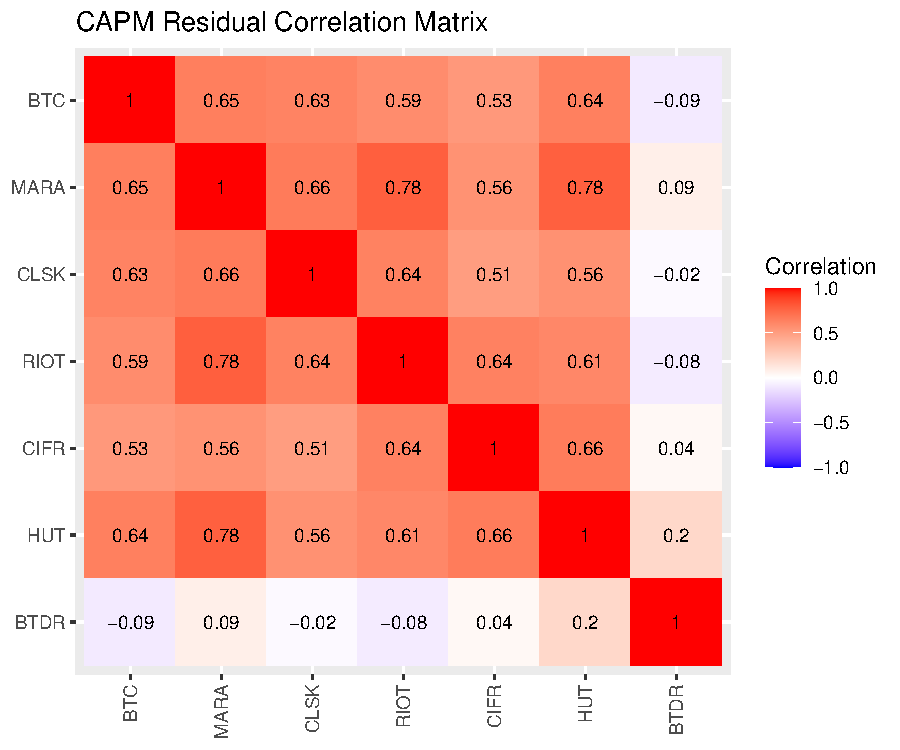
\includegraphics[width=\linewidth]{capm_resid_corplot.pdf}
\end{figure}

\subsection{Model (2): CAPM + BTC}

\begin{figure}[htbp]
	\label{bfm_resid_corplot}
	\caption{Correlation Matrix Heatmap for CAPM+BTC Residuals}
	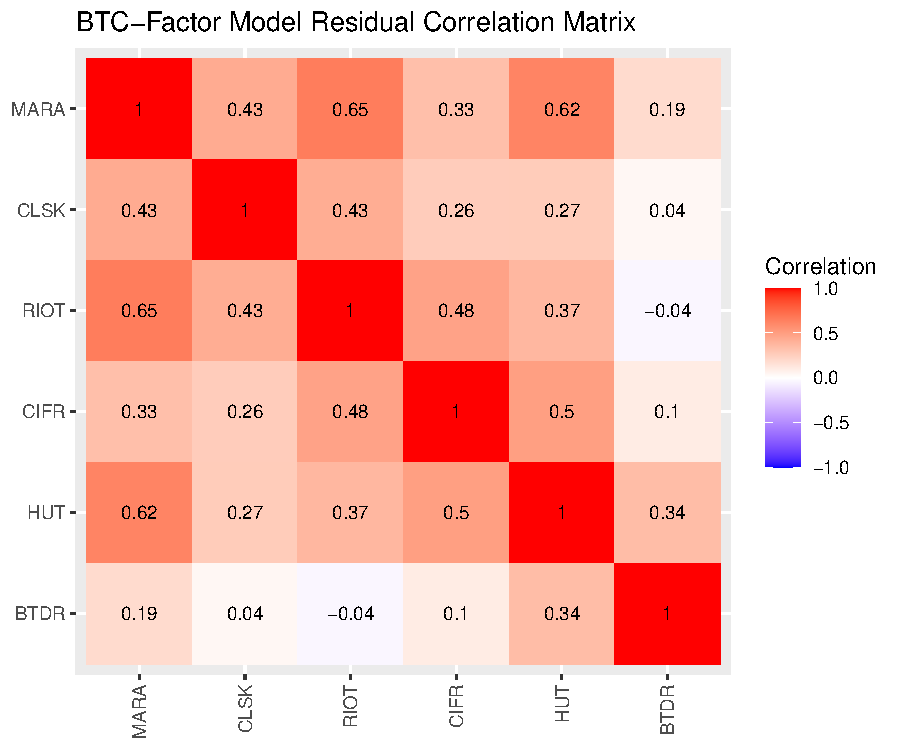
\includegraphics[width=\linewidth]{bfm_resid_corplot.pdf}
\end{figure}



\end{document}
